%--------------------
% Packages
% -------------------
\documentclass[11pt,a4paper]{article}
\usepackage[utf8x]{inputenc}
\usepackage[T1]{fontenc}
%\usepackage{gentium}
\usepackage{mathptmx} % Use Times Font
\usepackage{amsmath}

\usepackage[pdftex]{graphicx} % Required for including pictures
\graphicspath{ {images/} }
\usepackage[pdftex,linkcolor=black,pdfborder={0 0 0}]{hyperref} % Format links for pdf
\usepackage{calc} % To reset the counter in the document after title page
\usepackage{enumitem} % Includes lists

\frenchspacing % No double spacing between sentences
\linespread{1.2} % Set linespace
\usepackage[a4paper, lmargin=0.1666\paperwidth, rmargin=0.1666\paperwidth, tmargin=0.1111\paperheight, bmargin=0.1111\paperheight]{geometry} %margins
%\usepackage{parskip}

\usepackage[all]{nowidow} % Tries to remove widows
\usepackage[protrusion=true,expansion=true]{microtype} % Improves typography, load after fontpackage is selected

\counterwithin*{subsection}{section}
\renewcommand{\thesubsection}{\thesection.\alph{subsection}}

%-----------------------
% Set pdf information and add title, fill in the fields
%-----------------------


\hypersetup{ 	
pdfsubject = {Machine Learning 2 - Final Assignment},
pdftitle = {Machine Learning 2 - Final Assignment},
pdfauthor = {Frans de Boer}
}

\title{Machine learning 2 - Final Assignment}

\author{
    Frans de Boer \\
    frans.deboer \\
    5661439 \\
}

%-----------------------
% Begin document
%-----------------------
\begin{document} %All text i dokumentet hamnar mellan dessa taggar, allt ovanför är formatering av dokumentet
\maketitle

The git repository for this assignment (including code and the report) can be found at github.com. I will make this repository public after the Brightspace deadline has passed.

\section{PAC Learning}

\subsection{Extend the proof that was given in the slides for the PAC-learnability of hyper-rectangles:
show that axis-aligned hyper-rectangles in n-dimensional feature spaces (n > 2) are PAC
learnable.}
  
We can extend the proof by taking the number of sides/faces of the hyper-rectangle into account.
\begin{itemize}
    \item A hyper-rectangle in 2-dimensional space is simply a rectangle and has 4 sides.
    \item A hyper-rectangle in 3-dimensional space is a rectangular box and has 6 sides.
\end{itemize}
For now I will assume the number of sides on a n-dimensional hyper-rectangle to be $F(n)$, and I will get back later to the calculation of $F(n)$.

To start we can follow the steps from the lecture. We have the ground truth n-dimensional hyper-rectangle $R$, and the current tightest fit rectangle $R'$. The error ($R - R'$) can be split into $F(n)$ strips $T'$. On each of these strips we can now grow a new strip $T$ such that the probability mass of $T$ is $\frac{\epsilon}{F(n)}$.

If $T$ covers $T'$ for all strips then the probability of an error is
\begin{equation}
    \label{eq:total_error}
    P[error] \leq \sum_{i=0}^{F(n)-1}P[T_i] = F(n)\frac{\epsilon}{F(n)} = \epsilon
\end{equation}

We can now estimate the probability that $T$ does not cover $T'$

\begin{align*} 
    &P[\textit{random x hits T}] = \frac{\epsilon}{F(n)} \\
    &P[\textit{random x misses T}] = 1 - \frac{\epsilon}{F(n)} \\
    &P[\textit{m random x's misses T}] = (1 - \frac{\epsilon}{F(n)})^m \\
\end{align*}

Since we have $F(n)$ strips:
\begin{align*} 
    &P[\textit{m random x's miss any Ts}] \leq F(n) (1 - \frac{\epsilon}{F(n)})^m \\
    &P[\textit{R' has larger error than } \epsilon] \leq F(n) (1 - \frac{\epsilon}{F(n)})^m\ < \delta \\
\end{align*}

Bounding the chance that our R' has an error larger than $\epsilon$ by $\delta$:

\[F(n) (1 - \frac{\epsilon}{F(n)})^m\ < \delta\]
Using $e^{-x} \geq (1-x)$
\[F(n)e^{-m\epsilon / F(n)} \geq F(n)(1 - \frac{\epsilon}{F(n)})^m\]
So instead we can use:

\begin{align*} 
    &F(n)e^{-m\epsilon / F(n)} < \delta \\ 
    &-m\epsilon / F(n) < \log{(\delta / F(n))} \\
    &m\epsilon / F(n) > \log{(F(n) / \delta)} \\
    &m > (F(n) / \epsilon)\log{(F(n) / \delta)} \\
\end{align*}

So any n-dimensional hyper-rectangle is learnable.

\subsection{Assume we have a 2-dimensional feature space R2, and consider the set of concepts that are L1-balls: $c = \{(x, y) : |x| + |y| ≤ r\}$ (basically, all L1-balls centered around the origin). Use a learner that fits the tightest ball. Show that this class is PAC-learnable from training data of size m.}

Same thing? what. literally just question a but now rotated 45 degrees

\subsection{Now we extend the previous class by allowing the varying center: $c = \{(x, y) : |x − x0| + |y − y0| ≤ r\}$. Is this class PAC-learnable? Proof if it is, or otherwise disproof it.}

maybe, maybe not. can't you still just do the tightest fit L1 ball?
consistent learner so PAC learnable?

\clearpage
\section{VC Dimension}
\label{sec:VC}
Let us assume we are dealing with a two-class classification problem in d-dimensions.
Let us start off with refreshing our memories. Consider the class of linear hypotheses (i.e.,
all possible linear classifiers) in d-dimensional space.

\subsection{Given N data points, how many possible labelings does this data set have?}
\label{sec:2a}
Each data point can have 2 labels, so $2^N$

\subsection{What is the dimensionality d we need, at the least, for our class of linear hypotheses to
be able to find perfect solutions to all possible labelings of a data set of size N? Stated
differently, what is the smallest d that allows us to shatter N points?}
\label{sec:2b}
$d - 1$ 


\subsection{Consider d = 1 and a data set of size N. At maximum, how many different labelings of
such a data set can decision stumps solve perfectly, i.e., with zero training error?}
\label{sec:2c}
This would be all cases where there is no overlap, i.e. all points with class 1 (or 2) are either all on the left or right side. See Figure \ref{fig:d1n3} for an example with N=3. Note that the first 3 and last 3 examples are the same, just with inverted labelings.

\begin{figure}[h]
    \caption{Example of perfectly solvable labels with $N=3$}
    \centering
    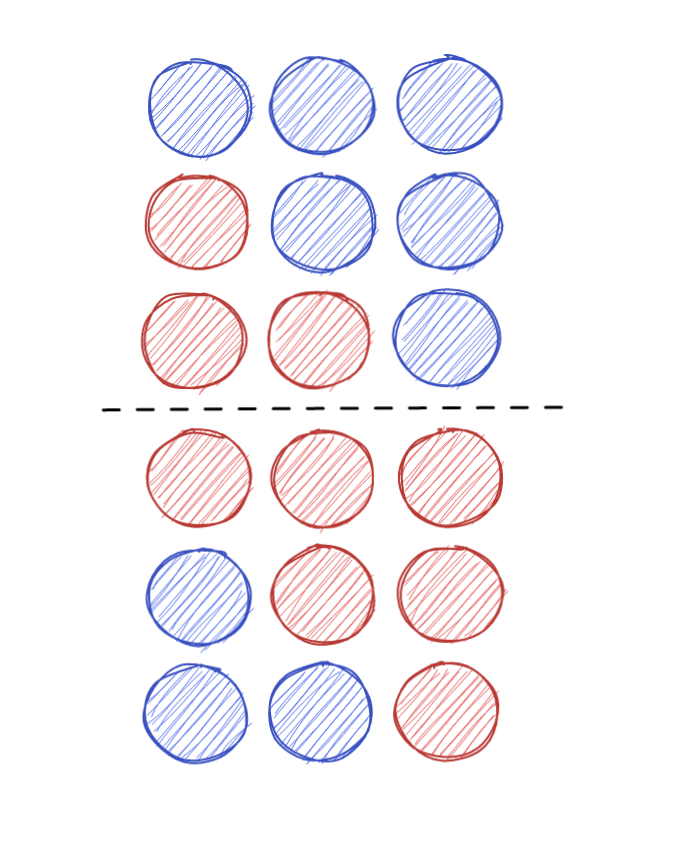
\includegraphics[width=0.5\textwidth]{d1n3_possibilities.png}
    \label{fig:d1n3}
\end{figure}

With a dataset of size N, there are N ways in which we can have class 1 be on the left side and have a decision stump be able to solve it perfectly. There can be $1, 2, ..., N$ points with class 1 in a row.
Because each of these possible label assignments has a compliment (just invert the classes), we end up with a total of $2N$ possible labelings that a decision stump can solve perfectly.


\subsection{With the answer from 3.c, give an upper-bound on the maximum number of different
labelings a data set of size N in d dimensions can get by means of decision stumps.}
\label{sec:2d}

We can once again look at Figure \ref{fig:d1n3}, but now instead of true labels we can view the labels (red and blue) as labels predicted by the decision stump. The decision stump either assigns all points to the left of it as class 1 or as class 2. So in $d=1$ we know the maximum number of different labelings a data set of size N can get is $2N$. 

This can be viewed in another way, for every dimension the decision stump can make $2N$ different labelings. For example in 2D (Figure \ref{fig:d2n3}) the decision stump for the x dimension can make $2N$ labelings, and the decision stump for the y dimension can make $2N$ labelings.

This continues for each dimension added, so we end up with a total of $2Nd$ maximum number of different labelings a data set of size N in d dimension can get by means of decision stumps.


\begin{figure}[h]
    \caption{Example with $d=2$ and $N=3$}
    \centering
    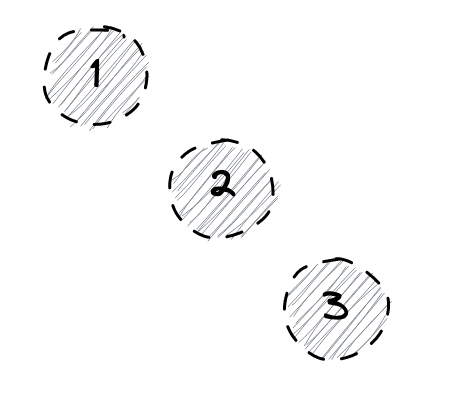
\includegraphics[width=0.5\textwidth]{d2n3_unlabeled.png}
    \label{fig:d2n3}
\end{figure}

I'd like to add some more notes to this solution. This is not neccesary to read, but it sheds some light on the work I did for this question and some of the mistakes I made. 

While trying to answer this question I pretty quickly came to the answer of $2Nd$, but then later thought it to be wrong because this formula does not take into account duplicate labelings. In Figure \ref{fig:d2n3} for example the x and y decision stumps can create many duplicate label assignments. 

I tried to find patterns in combinations of $N$ and $d$, for example I noticed that for $d=2$ only $N \leq 3$ was solvable (see Figure \ref{fig:d2n3_solvable}), and for $d=3$ at least $N \leq 4$ was solvable (see Figure \ref{fig:d3n4_solvable}, here smaller circles can be seen as being further away in the z dimension). 

From here it seemed like there was a pattern where for any $N \leq (d+1)$ the problem was fully solvable, so the number of possible labelings the decision stump could make was $2^N$. I could however not find a pattern in the number of labelings a decision stump could make for problems with $N > (d+1)$.

\begin{figure}[h]
    \caption{Solvable example with $d=2$ and $N=3$}
    \centering
    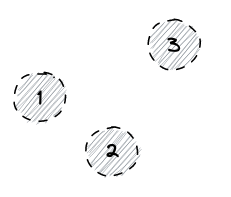
\includegraphics[width=0.5\textwidth]{d2n3_solvable.png}
    \label{fig:d2n3_solvable}
\end{figure}

\begin{figure}[h]
    \caption{Solvable example with $d=3$ and $N=4$}
    \centering
    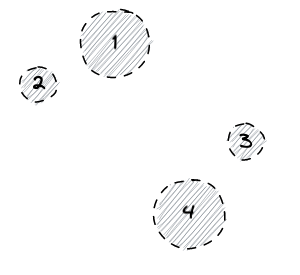
\includegraphics[width=0.5\textwidth]{d3n4_solvable.png}
    \label{fig:d3n4_solvable}
\end{figure}


It was not until a day of thinking and researching that I found these \href{https://people.csail.mit.edu/alinush/6.867-fall-2013/2013.10.22.w8.tu-lecture-13-generalization-part-2.pdf}{Slides} (Page 5) that confirmed my original answer.

\subsection{Using the bound from Exercise 3.d, determine the smallest upper-bound on the VC-dimension for decision stumps for dimensionalities $d ∈ \{1, 2, 3, 4, 5, 6, 7, 8, 1024, 2^{100}\}$}
\label{sec:3e}
I used the definition from the book \textit{Foundations of Machine Learning} \cite{foundations_of_machine_learning} for the upper-bound on the VC-Dimension
\textbf{Smallest upper-bound}: To give an upper bound, we need to prove that no set $S$ of cardinality $N$ can be shattered

Since we know the maximum number of different labelings a data set of size $N$ in $d$ dimensions can get by means of decision stumps to be $2Nd$ (Section \ref{sec:2d}), and the total number of possible different labelings of a data set of size $N$ can get is $2^N$ (Section \ref{sec:2a}), we have to find the first case where $2Nd < 2^N$. In other words, find the first $N$ for which the classifier cannot create every possible labeling.

Since I could not find an analytical solution to this I decided to solve it programmatically. The results can be seen in Table \ref{tab:upper-bound-vc}.

\begin{table*}
    \begin{tabular}{|c|c|}
    \hline
    Dimensionality & Upper-bound on VC-Dimension \\ \hline
    1              & 2                            \\ \hline
    2              & 4                            \\ \hline
    3              & 4                            \\ \hline
    4              & 5                            \\ \hline
    5              & 5                            \\ \hline
    6              & 6                            \\ \hline
    7              & 6                           \\ \hline
    8              & 6                            \\ \hline
    1024           & 14                            \\ \hline
    $2^{100}$        & 107 \\
    \hline
    \end{tabular}
    \caption{Results for upper bounds on the VC Dimension}
    \label{tab:upper-bound-vc}
\end{table*}

To me one interesting thing about these results is that they did not seem to agree with some other results I had found online. \href{https://people.csail.mit.edu/alinush/6.867-fall-2013/2013.10.22.w8.tu-lecture-13-generalization-part-2.pdf}{These slides} mentions the growth should be proportional to $\log(d)$, which it is. But \href{http://courses.cms.caltech.edu/cs253/hw/hw2.pdf}{This homework assignment} gives an upper bound on the VC dimension of $2(\log_2(d) + 1)$. 

\bibliographystyle{plain}
\bibliography{refs}

\end{document}